\documentclass[10pt,journal,compsoc]{IEEEtran}
\usepackage{graphicx, soul} 
\usepackage{soul} % soul pachage must be removed when the paper is ready
\usepackage{colortbl} % Biblioteca para el color
\usepackage{color} % Biblioteca para el color
\usepackage{xcolor} % Biblioteca para el color

\usepackage{listings}
\usepackage{hyperref}

%% A number of IDs used in authentication protocols
\newcommand{\lnk}{;}
\newcommand{\QR}{Qr}

%% Operators
\newcommand{\keysFor}{\textsf{keysFor}\;}
\newcommand{\invKey}{\textsf{invKey}\;}

%% Message items

\newcommand{\Agent}{\textsf{Agent}\;}
\newcommand{\Number}{\textsf{Number}\;}
\newcommand{\Key}{\textsf{Key}\;}
\newcommand{\Nonce}{\textsf{Nonce}\;}
\newcommand{\Hash}{\textsf{Hash}\;}
\newcommand{\Crypt}{\textsf{Crypt}\;}
\newcommand{\Xor}{\textsf{Xor}}

%% Rôles

\newcommand{\initiator}{\textrm{initiator}} 
\newcommand{\responder}{\textrm{responder}}

%% Events and messages

\newcommand{\msg}{\mathsf{msg}}

%% Agents, server, etc.
\newcommand{\Friend}{\textsf{Friend}\;}
\newcommand{\Spy}{\textsf{Spy}}
\newcommand{\Server}{\textsf{M}}
\newcommand{\ServerW}{\textsf{M}_{W}}
\newcommand{\Servera}{\textsf{S}_{CA}}
\newcommand{\Client}{\textsf{C}}
\newcommand{\server}{\textsf{Server}\;}

%% Event operators

\newcommand{\knows}{\textsf{knows}\;}
\newcommand{\knowsSpy}{\textsf{knows}\,_{\textsf{\tiny Spy}}\:}
\newcommand{\knowsF}{\textsf{knows}\,_{\textsf{\tiny Friend}}\:}
\newcommand{\initState}{\textsf{initState}\;}
\newcommand{\bad}{\textsf{bad}\;}

%% def operator
\newcommand{\Def}{\stackrel{\rm def}{=}}

%% BAN constructors


%% Needham constructors
\newcommand{\nsPub}{\textsf{ns\_public}\;} 
\newcommand{\evsone}{\textsf{evs1}}
\newcommand{\evstwo}{\textsf{evs2}}
\newcommand{\evsthree}{\textsf{evs3}}


\newcommand{\fat}[1]{\left\{\hspace*{-0.03in}\left|{#1}\right|\hspace*{-0.03in}\right\}}

\newcommand{\lfat}[1]{\left\{\!\arrowvert{#1}\right.}
\newcommand{\rfat}[1]{\left.{#1}\arrowvert\!\right\}}

%\newcommand{\fat}[1]{\lbrace\!|{#1}|\;\,\,\!\!\!\!\rbrace}
\newcommand{\cons}{\,\#\,}

%Stega constructors
\newcommand{\As}{\textsf{AE}\;}

%% equal2Eyes operator
\newcommand{\eqToEyes}{\stackrel{\odot}{\approx}}

\ifCLASSOPTIONcompsoc
 \usepackage[nocompress]{cite}
\else
  \usepackage{cite}
\fi

\ifCLASSINFOpdf
\else
\fi
\hyphenation{Blockchain and smart contracts}

\begin{document}
        \newcommand{\blockchaincarnetwork}{\textit{vehicle blockchain network~}}
        \newcommand{\duda}[1]{\textcolor{red}{\textit{#1}}}

        \begin{frontmatter}

%% Title, authors and addresses

%% use the tnoteref command within \title for footnotes;
%% use the tnotetext command for theassociated footnote;
%% use the fnref command within \author or \address for footnotes;
%% use the fntext command for theassociated footnote;
%% use the corref command within \author for corresponding author footnotes;
%% use the cortext command for theassociated footnote;
%% use the ead command for the email address,
%% and the form \ead[url] for the home page:
%% \title{Title\tnoteref{label1}}
%% \tnotetext[label1]{}
%% \author{Name\corref{cor1}\fnref{label2}}
%% \ead{email address}
%% \ead[url]{home page}
%% \fntext[label2]{}
%% \cortext[cor1]{}
%% \address{Address\fnref{label3}}
%% \fntext[label3]{}




%\title{A Distributed Model to Store Vehicle Transaction Records Through Blockchain Platform}
\title{Towards a Distributed Network Model to Store Vehicle Transaction Records Through Blockchain Platform}
%% use optional labels to link authors explicitly to addresses:
%% \author[label1,label2]{}
%% \address[label1]{}
%% \address[label2]{}

\author{Juan-Carlos L\'opez-Pimentel,
        Miguel Alcaraz Rivera,
        %~\IEEEmembership{Fellow,~OSA,},
        Leonardo J. Valdivia,
        and Carolina del Valle Soto% <-this % stops a space
}

\address{}

\begin{abstract}
%% Text of abstract
Blockchain technology, from its emergence until now, has been applied to several projects and 
not just for cryptocurrencies. 
Although this technology has been used for several challenges, to our knowledge, there are no 
records of having applied it to smart properties in vehicles.
In this work, we present a transaction based solution to handle motorized vehicles ownership 
and provenance. 
The solution is based on a distributed model using smart properties and blockchain technologies,  
which offers a secure and useful system where transactions can be requested to handle, 
validate and update the vehicle information. 
The model includes the specification of various client-server security protocols verified formally using AVISPA-SPAN tool.  
The client can have different roles accordingly to the relationship it has with the 
physical property and it can get services and request transactions;
meanwhile the \blockchaincarnetwork  acts as the server entity. 
%Some transaction examples are shown. 
We believe that our proposal can contribute to reduce frauds and increase the trend of 
paperless culture that is strongly being promoted in recent years.

%We present a transaction based solution to handle motorized vehicles ownership 
%and provenance over a distributed model using smart contracts,  
%including the specification of client-server security protocols,
%roles, services, transactions and the \blockchaincarnetwork acting as server.
%Our proposal will reduce frauds and increase the trend of paperless culture.
  %  %Blockchain technology, from its emergence until now, has been applied to several projects and 
%not just for cryptocurrencies. 
%Although this technology has been used for several challenges, to our knowledge, there are no 
%records of having applied it to smart properties in vehicles.
%In this work, we present a transaction based solution to handle motorized vehicles ownership 
%and provenance. 
%The solution is based on a distributed model using smart properties and blockchain technologies,  
%which offers a secure and useful system where transactions can be requested to handle, 
%validate and update the vehicle information. 
%The model includes the specification of various client-server security protocols.  
%The client can have different roles accordingly to the relationship it has with the 
%physical property and it can get services and request transactions;
%meanwhile the \blockchaincarnetwork  acts as the server entity. 
%%Some transaction examples are shown. 
%We believe that our proposal can contribute to reduce frauds and increase the trend of 
%paperless culture that is strongly being promoted in recent years.

We present a transaction based solution to handle motorized vehicles ownership 
and provenance over a distributed model using smart contracts,  
including the specification of client-server security protocols,
roles, services, transactions and the \blockchaincarnetwork acting as server.
Our proposal will reduce frauds and increase the trend of paperless culture.
\end{abstract}

\begin{keyword}
%% keywords here, in the form: keyword \sep keyword
Smart contract 
\sep Smart property
\sep Blockchain
\sep Cloud Computing
\sep Security Protocols
%% PACS codes here, in the form: \PACS code \sep code

%% MSC codes here, in the form: \MSC code \sep code
%% or \MSC[2008] code \sep code (2000 is the default)

\end{keyword}

\end{frontmatter}

        
        %\tableofcontents    % this line must be removed
        
       % \section{Introduction}
The paperless culture extends throughout the world. 
From the birth of the scanner to the invention of cloud computing, 
technology has been making its way into business processes 
with the aim of facilitating operations and reducing the use of paper, 
for both economic and environmental reasons. 

Companies and organizations who seek to become paperless can increase the automation of their processes and at the same time use a minimum amount of paper.
At a bigger scale, this is not a complete process and in some cases is not even encouraged.
Even today, 
in some communities where an electronic bill is required when selling goods, 
it has to be printed afterwards and then officially signed, 
via holograms or stamps, 
for it to become a legal proof. 

The combination of electronic and physical documents introduces some application problems, 
like a lack of clarity in the process of passing ownership.
Specially troublesome is the case when the goods are expensive, like automobiles.
Sometimes, a car is the most valuable possession a person has, 
making the selling process a subject of constant scrutiny 
because if a fraud is committed in the exchange, 
the affected party can lose a big fraction of its patrimony.

To solve our challenge, a recent technology called smart property can be used. 
It is a specialization of 
smart contracts supported by the blockchain technology.
%Examples could include physical property such as vehicles, phones or houses. 
A smart contract is a computer protocol intended to digitally facilitate,
verify, or enforce the negotiation or performance of a
contract, using transactions. These transactions are traceable
and irreversible.

%In this paper, 
%we will present a distributed model solution based on smart properties technology 
%to handle automobile related transactions 
%that offers a secure, useful and easy to use system on which car ownership can be
%handled, validated and updated.

In this paper, 
we present a distributed model solution based on smart properties technology 
to handle automobile related transactions on which vehicle ownership, 
among others, can be handled, validated and updated through a 
secure and useful system with traceable and irreversible characteristics. 
Our model is presented as a lot of security protocols, each of them is shown
in Alice and Bob notation.

The paper is organized as follows: 
First, in Section~\ref{sec:background}
we look at recent technologies that can handle this kind of system,
like blockchain, smart contracts and smart properties; and some related works.
Then, in Section~\ref{sec:outline}
we propose a model to control vehicle transactions through blockchain network platform 
that at the same time will prevent fraudulent operations. 
%Our model starts by car dealerships including a QR code in vehicles. 
%The code could be read by users who can use it to do transactions through 
%the vehicle blockchain network. 
Sections~\ref{sec:client},~\ref{sec:getServices} and~\ref{sec:transactions} presents the model 
we are proposing with a step by step explanation. 
%using Alice and Bob notation to explain our general model.
%the invoice supply-chain provenance. 
Finally, our conclusions are given.
        %\subsection{Case Study}
Before 2014 the legal procedure of selling a vehicle in Mexico is described in the following
work flow:
\begin{enumerate}
    \item The buyer might check that no legal problems are involved with the vehicle. 
          An online check can be done with the plate number. 
    \item The buyer makes the car payment.
    \item The seller endorses his bill to the new owner and gives possession of the car 
    to the buyer.
    %generates an electronic bill for the value of the car and acknowledges payment from the buyer
    \item The change of ownership is notified to the city government. In some cities a 
        change of plates is necessary and a new set of plates is given to the new owner.
\end{enumerate}

From 2012, Mexico joins the paperless culture in the world,\footnote{The introduction of the Advance
Electronic Signature published by the Official Journal of the Federation via \url{https://www.dof.gob.mx/nota_detalle.php?codigo=5228864&fecha=11/01/2012}} 
but from 2014, paper bills stopped being a legal proof of ownership. 
This led to some problems in the purchase procedure.

Using the electronic bill with the above work flow provides a vulnerability between steps $2$ and $3$. 
Step $2$ can be generated even without the existence of a physical car. A malicious seller 
could generate multiple apparently original bills and give to multiple buyers before 
they realize the car doesn't exist physically. A certain level of \textit{trust} must 
exist between buyer and seller for the exchange to happen. And this \textit{trust} can be 
maligned. 

This fraud is specially common on car sales between private owners for a couple reasons. 
The first one is the high value of this commodity, which makes it a low risks - high stakes 
trade-off for fraudsters. The other one comes with the definition of car: a portable, efficient, 
and maneuverable transportation vehicle that can be easily removed from the transaction scene 
and hidden afterwards.

Due to the lack of immediate retaliation available to the criminal, he has a time frame where 
the fraud could be repeated multiple times, even if finally, the car exchange takes place with 
an Innocent buyer afterwards.

Currently, the solution proposed by dealerships have been to sign officially a physical 
invoice (see Figure~\ref{fig:invoice} for an example) including holograms (left side
in the figure), a stamp (right side, below of the signature) and a QR code (below on the
right side). 
However, it falls back again into a paper culture. We have revised that the case 
study exposed in this section is also active in several countries.
\begin{figure}[hbt]
 %\begin{center}
  \centering
    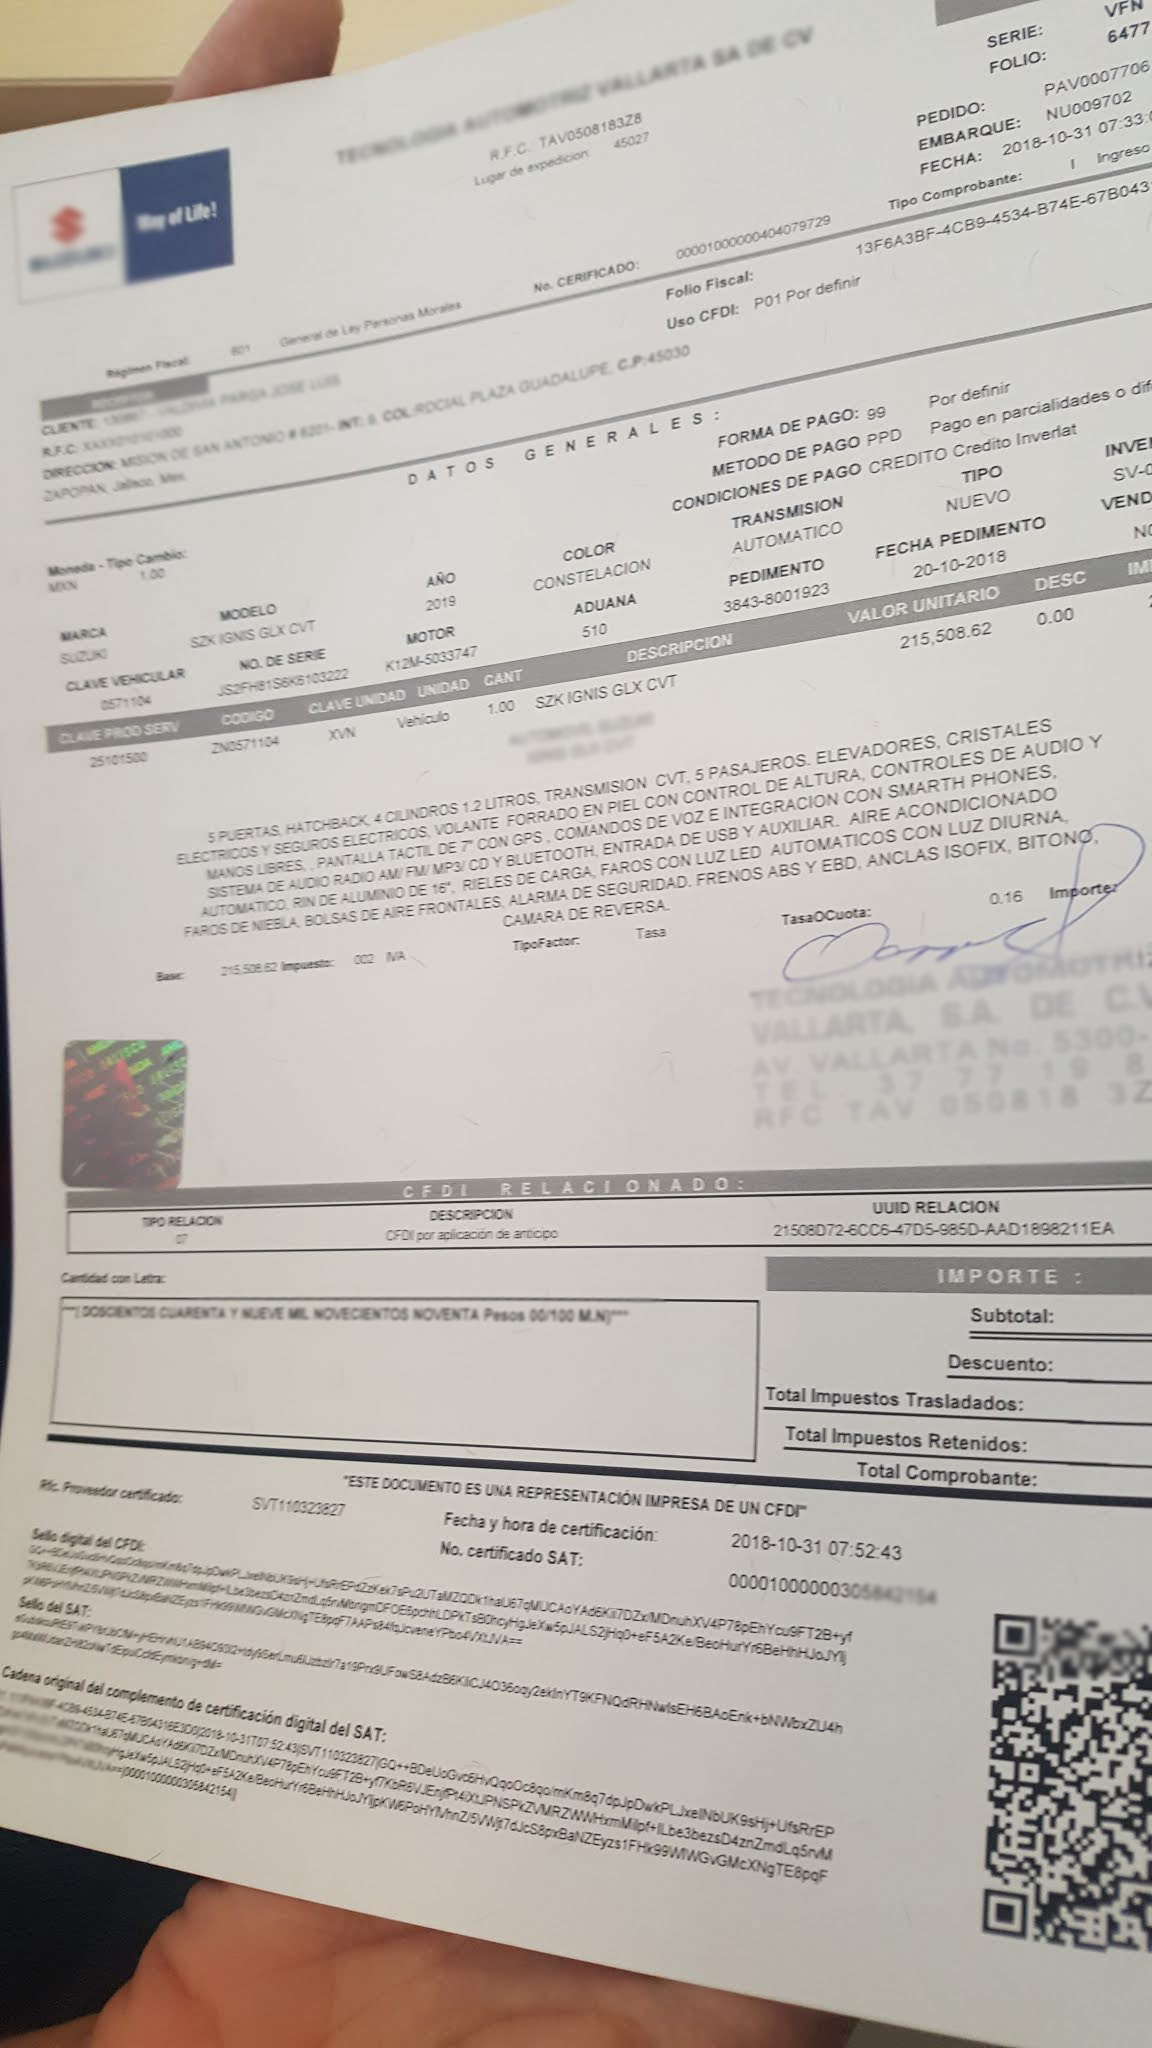
\includegraphics[scale=0.4]{images/lopez1.png}
        \caption{Formal Invoice including a hologram, a stamp and a signature}
    \label{fig:invoice}
 % \end{center}
\end{figure}


        %\section{Client roles}

According to the permissions the clients should have, there will be three defined roles for them:

\begin{enumerate}
    \item Querier
    \item Owner
    \item Helper
    \item Law enforcer
\end{enumerate}

The querier will have permissions sufficient to interact with the system in order to query and obtain information on the vehicle. This permissions will be granted to the querier once the client is able to establish a secure channel.

Every car will have one and only one owner at a given time. The owner will be the only client that has permission to trade ownership. 


The helper role is a client who receives a temporal permission from the owner to set one transaction on the block-chain. The time frame for the temporal permission will be allotted by the owner of the car. The car owner will set a special transaction to give the helper the permission. 
The helper role will be used for transactions that change the value of the property. This will include official services, mechanical adjustments, big aesthetic modifications and insurance payments.

The law enforce roles will have the ability to change the value of the car when the vehicle is involved in legal situations. It won’t need the permission of the owner to modify the status.
        \section{Introduction}
The paperless culture extends throughout the world. 
From the birth of the scanner to the invention of cloud computing, 
technology has been making its way into business processes 
with the aim of facilitating operations and reducing the use of paper, 
for both economic and environmental reasons. 

Companies and organizations who seek to become paperless can increase the automation of their processes and at the same time use a minimum amount of paper.
At a bigger scale, this is not a complete process and in some cases is not even encouraged.
Even today, 
in some communities where an electronic bill is required when selling goods, 
it has to be printed afterwards and then officially signed, 
via holograms or stamps, 
for it to become a legal proof. 

The combination of electronic and physical documents introduces some application problems, 
like a lack of clarity in the process of passing ownership.
Specially troublesome is the case when the goods are expensive, like automobiles.
Sometimes, a car is the most valuable possession a person has, 
making the selling process a subject of constant scrutiny 
because if a fraud is committed in the exchange, 
the affected party can lose a big fraction of its patrimony.

To solve our challenge, a recent technology called smart property can be used. 
It is a specialization of 
smart contracts supported by the blockchain technology.
%Examples could include physical property such as vehicles, phones or houses. 
A smart contract is a computer protocol intended to digitally facilitate,
verify, or enforce the negotiation or performance of a
contract, using transactions. These transactions are traceable
and irreversible.

%In this paper, 
%we will present a distributed model solution based on smart properties technology 
%to handle automobile related transactions 
%that offers a secure, useful and easy to use system on which car ownership can be
%handled, validated and updated.

In this paper, 
we present a distributed model solution based on smart properties technology 
to handle automobile related transactions on which vehicle ownership, 
among others, can be handled, validated and updated through a 
secure and useful system with traceable and irreversible characteristics. 
Our model is presented as a lot of security protocols, each of them is shown
in Alice and Bob notation.

The paper is organized as follows: 
First, in Section~\ref{sec:background}
we look at recent technologies that can handle this kind of system,
like blockchain, smart contracts and smart properties; and some related works.
Then, in Section~\ref{sec:outline}
we propose a model to control vehicle transactions through blockchain network platform 
that at the same time will prevent fraudulent operations. 
%Our model starts by car dealerships including a QR code in vehicles. 
%The code could be read by users who can use it to do transactions through 
%the vehicle blockchain network. 
Sections~\ref{sec:client},~\ref{sec:getServices} and~\ref{sec:transactions} presents the model 
we are proposing with a step by step explanation. 
%using Alice and Bob notation to explain our general model.
%the invoice supply-chain provenance. 
Finally, our conclusions are given.
        \section{Background and Related Work}
\label{sec:background}

The introduction of digital smart contracts as an enforcement of accords eliminates the necessity of their written counterparts, contributing to a paperless culture. They also introduce a series of benefits, that makes them better than the latter, including digital data provenance. Smart contracts and their evolution to smart properties, are having a great push because the natural affinity they have to being implemented over blockchain technologies. 

The following subsections explain in detail the technologies described and closes with some platforms that are proposed to handle these tasks.

\subsection{Blockchain}

Blockchain technology can be abstracted to recall a series of blocks chained in series. In this abstraction, each block of the blockchain represents an object that records a transaction and the chaining is obtained by referencing the previously last block keeping track of the whole history starting from a first block, called \textit{genesis block}. Blockchain is a transaction record keeping platform that tries to attack a series of problems contained in other similar purpose platforms. It achieves its purposes by having the following features \cite{block}.

\begin{itemize}
\item Immutable: It is not possible for a given block to be modified without the agreement of the whole network.
\item Distributed system: Multiple copies of the blockchain exist among its members.
\item No centralized server: Blockchain does not depend on a central authority that dominates the system.            
\end{itemize}
Even though all these features are desired, when blockchain is mentioned as a solution is because of decentralization. Thus, giving control of the system to networks where the main beneficiaries are the users without necessarily having a government figure interested in controlling those exchanges, or where the users prefer to not involve third parties, due to the costs involved or the cumbersomeness of the extra steps required. 

The distribution and immutability of the chain also removes the trust component of a transaction \cite{iot}, i.e. making it a secure way to exchange titles of property between strangers.

\subsection{Data provenance}
Cloud computing allows the existence of digital representations of phyisical world objects in a permanent way, independent of a single copy existing on a specific location. This digital representation can contain information of the whole life cycle of the object, its accountability and historical changes. Specifically among cloud technologies, blockchain allows for the continuous existence of the digital representations introducing security aspects like traceability and resistance to unwanted modifications. Implementations have been made to preserve digital representations \cite{provchain}. Kim and Laskowski\cite{ontology} show an approach using Ethereum technology to propose ontologies that can represent knowledge provenance. The blockchain approach is having a great momentum in the data provenance medium for it theoretical strengths in security and data protection. Neisse et al. \cite{europe} give this a push by proposing enforcement of smart contracts to fulfill legal obligations of personal data over data controllers and processsors in Europe using blockchain. Blockchain provenance is not limited to storage information. Smart contracts inside the transactions allow for programmable interactive environments \cite{ramachandran} where the blockchain will be enriched with valid data and binding transactions every time something interesting happens to the physical part of the object.
\subsection{Smart Contracts}

A smart contract is a series of self-executing computer code that is fired when a transaction is trying to complete. These lines of code are part of the blockchain and allows for a series of conditions between the sender and receiver of the transaction to be completed before it succeeds. The whole process is completely automated without external help, requiring only the participation of the interested parties and the blockchain network.

The transaction itself can be a representation of a legal enforcement, and when used this way, should offer tamper-proofing to remove the possibility of bad use by either part, \cite{templates}.

The mechanism can be used as a secure way to enforce agreements using blockchain networks as support \cite{securing}.


%To solve our model, smart properties  is a recent technology that can be used to this. 
%Smart property is those whose ownership is controlled via block chain technology using 
%smart contracts~\cite{Tapscott2016}. Examples could include physical property such as 
%vehicles, phones or houses. A smart contract is a computer protocol intended to digitally 
%facilitate, verify, or enforce the negotiation or performance of a contract, using transactions. 
%These transactions are tractable and irreversible. 


\subsection{Platforms}
The existence of smart contracts over a blockchain expand the use cases of this revolutionary technology above its original use in Bitcoin, \cite{nakamoto}. As alternative to Bitcoin, other crytocurrency systems are continuously in development, and in some cases, their network also have processing power, to be consumed as a service for the users\cite{uses}. Among the multiple platforms with processing power that allow smart contract interactions a completely autonomous system can be modeled, working as a Decentralized Autonomous System \cite{dao}.
Complete autonomy is not yet implementable 
due to the nonexistence of a sufficiently mature smart contract environment, \cite{daofail}. Other similar systems use this full autonomous environment, like Slock.it, Augur, etc \cite{sense}. 

Specially among them Ethereum \cite{ethereum} as a platform also provides a full system where users can run custom-scripted code inside their transactions, embracing the idea of smart contracts over a decentralized medium. But in contrast with the ones mentioned before, Ethereum gives full control over the degree of autonomy required as a back technology that supports the development of this environment can be utilized to built a smart contract management system \cite{lazy}. 

Other options, like Hawk \cite{hawk} also allows for a fully customizable system, adding more benefits, like transactional privacy.


 %added by JC
        \section{Outline}
\label{sec:outline}
This section presents a case study explaining how
paperless culture is being limited by some fraud 
operations, then we outline a proposal and the notation used
throughout the document.


\subsection{Case Study}
Before 2014 the legal procedure of selling a vehicle in Mexico is described in the following
work flow:
\begin{enumerate}
    \item The buyer might check that no legal problems are involved with the vehicle. 
          An online check can be done with the plate number. 
    \item The buyer makes the car payment.
    \item The seller endorses his bill to the new owner and gives possession of the car 
    to the buyer.
    %generates an electronic bill for the value of the car and acknowledges payment from the buyer
    \item The change of ownership is notified to the city government. In some cities a 
        change of plates is necessary and a new set of plates is given to the new owner.
\end{enumerate}

From 2012, Mexico joins the paperless culture in the world,\footnote{The introduction of the Advance
Electronic Signature published by the Official Journal of the Federation via \url{https://www.dof.gob.mx/nota_detalle.php?codigo=5228864&fecha=11/01/2012}} 
but from 2014, paper bills stopped being a legal proof of ownership. 
This led to some problems in the purchase procedure.

Using the electronic bill with the above work flow provides a vulnerability between steps $2$ and $3$. 
Step $2$ can be generated even without the existence of a physical car. A malicious seller 
could generate multiple apparently original bills and give to multiple buyers before 
they realize the car doesn't exist physically. A certain level of \textit{trust} must 
exist between buyer and seller for the exchange to happen. And this \textit{trust} can be 
maligned. 

This fraud is specially common on car sales between private owners for a couple reasons. 
The first one is the high value of this commodity, which makes it a low risks - high stakes 
trade-off for fraudsters. The other one comes with the definition of car: a portable, efficient, 
and maneuverable transportation vehicle that can be easily removed from the transaction scene 
and hidden afterwards.

Due to the lack of immediate retaliation available to the criminal, he has a time frame where 
the fraud could be repeated multiple times, even if finally, the car exchange takes place with 
an Innocent buyer afterwards.

Currently, the solution proposed by dealerships have been to sign officially a physical 
invoice (see Figure~\ref{fig:invoice} for an example) including holograms (left side
in the figure), a stamp (right side, below of the signature) and a QR code (below on the
right side). 
However, it falls back again into a paper culture. We have revised that the case 
study exposed in this section is also active in several countries.
\begin{figure}[hbt]
 %\begin{center}
  \centering
    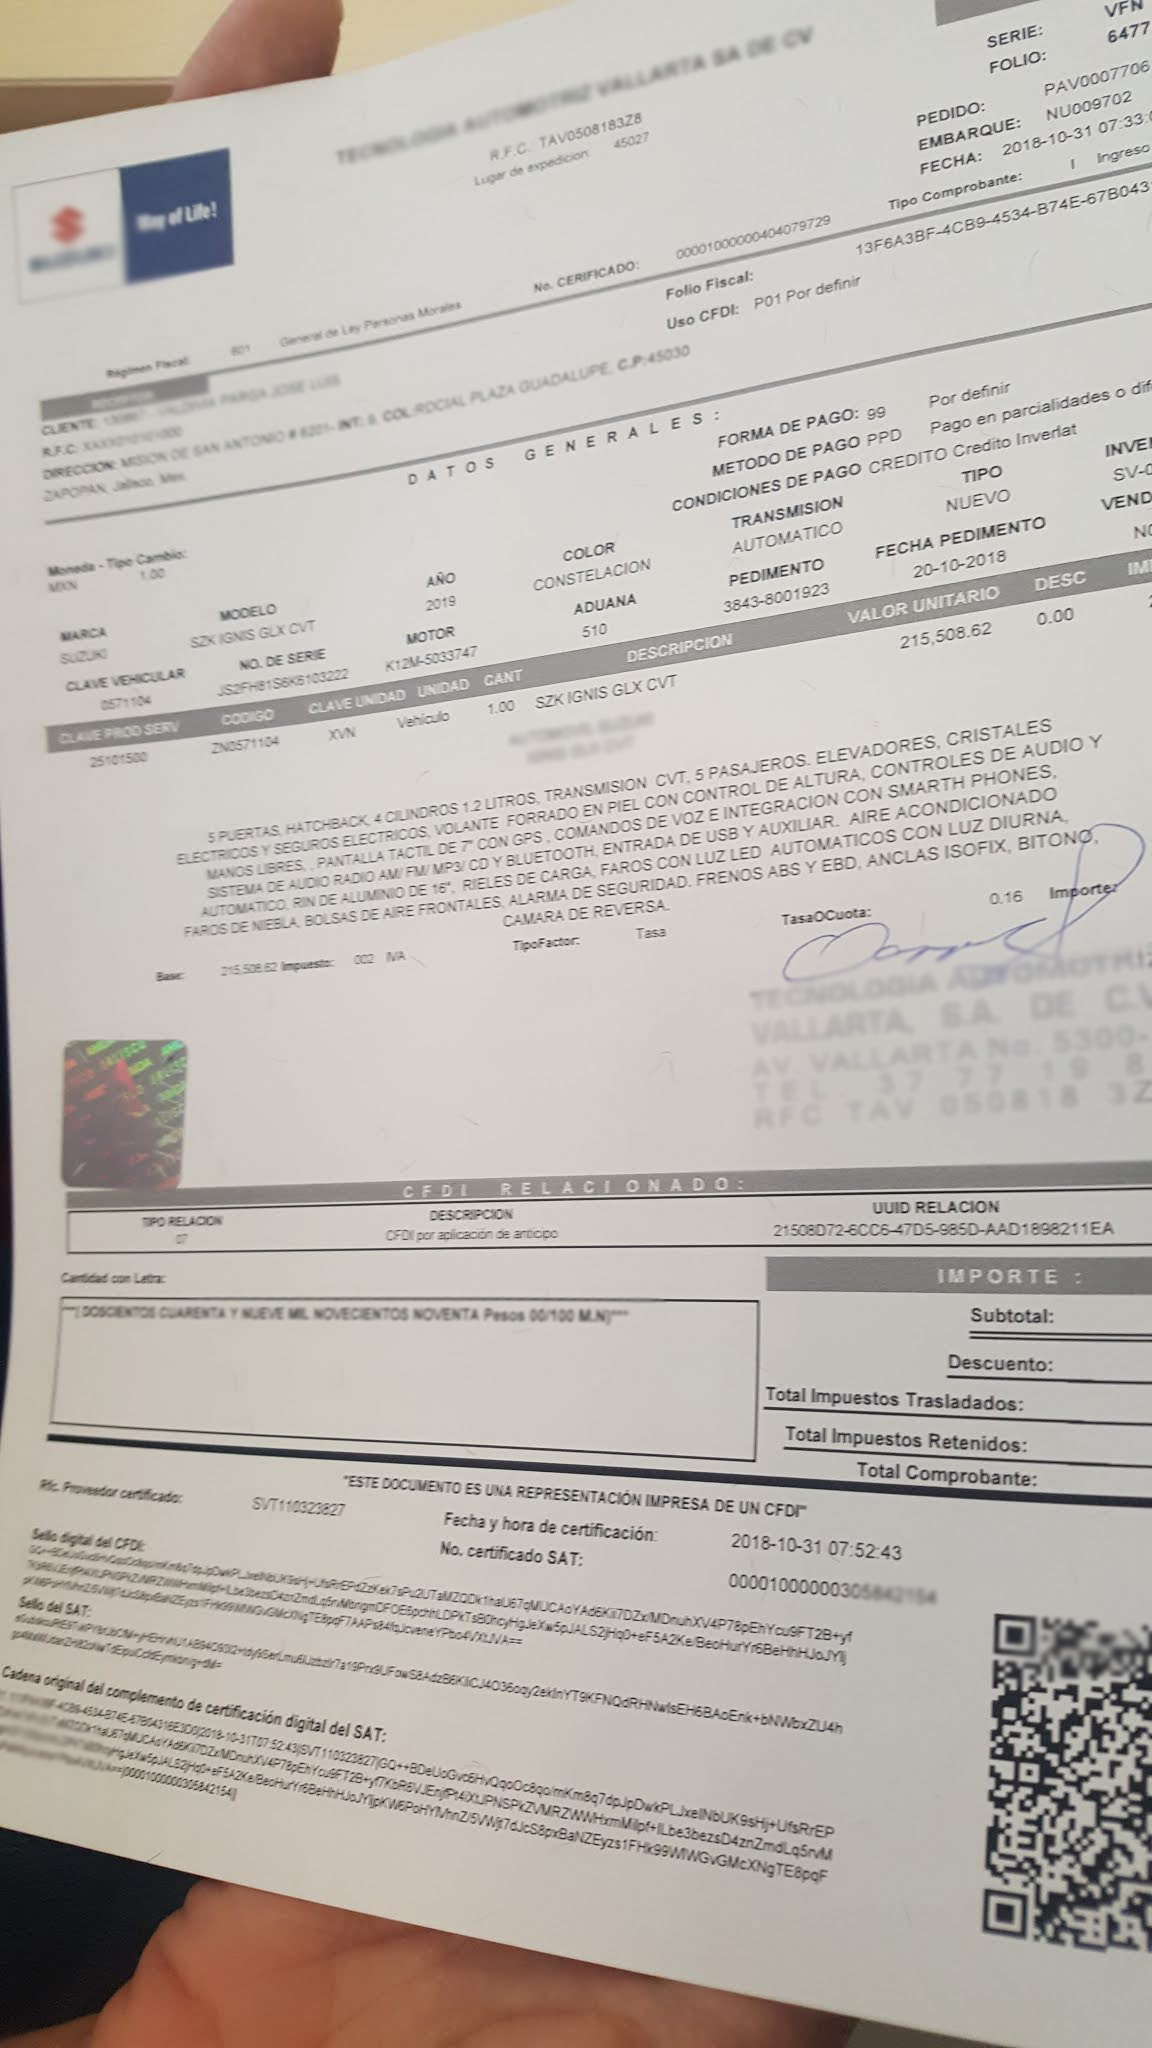
\includegraphics[scale=0.4]{images/lopez1.png}
        \caption{Formal Invoice including a hologram, a stamp and a signature}
    \label{fig:invoice}
 % \end{center}
\end{figure}


\subsection{Proposal}
\label{subsec:proposal}
In general there exists some characteristics, in the vehicles, we are looking for:
a) Provenance,
b) Transparency with respects to purchase sale,
c) Traceability with history transactions, owners and legal situations (including  
government participation).

To achieve these goals, we have proposed a distributed model illustrated in the context
diagram in Figure~\ref{fig:flowChartFramework}. Such a figure denotes
the general stages (circled numbers) a user must follow to get or set information about a 
vehicle:
\begin{figure}[hb]
 %\begin{center}
  \centering
    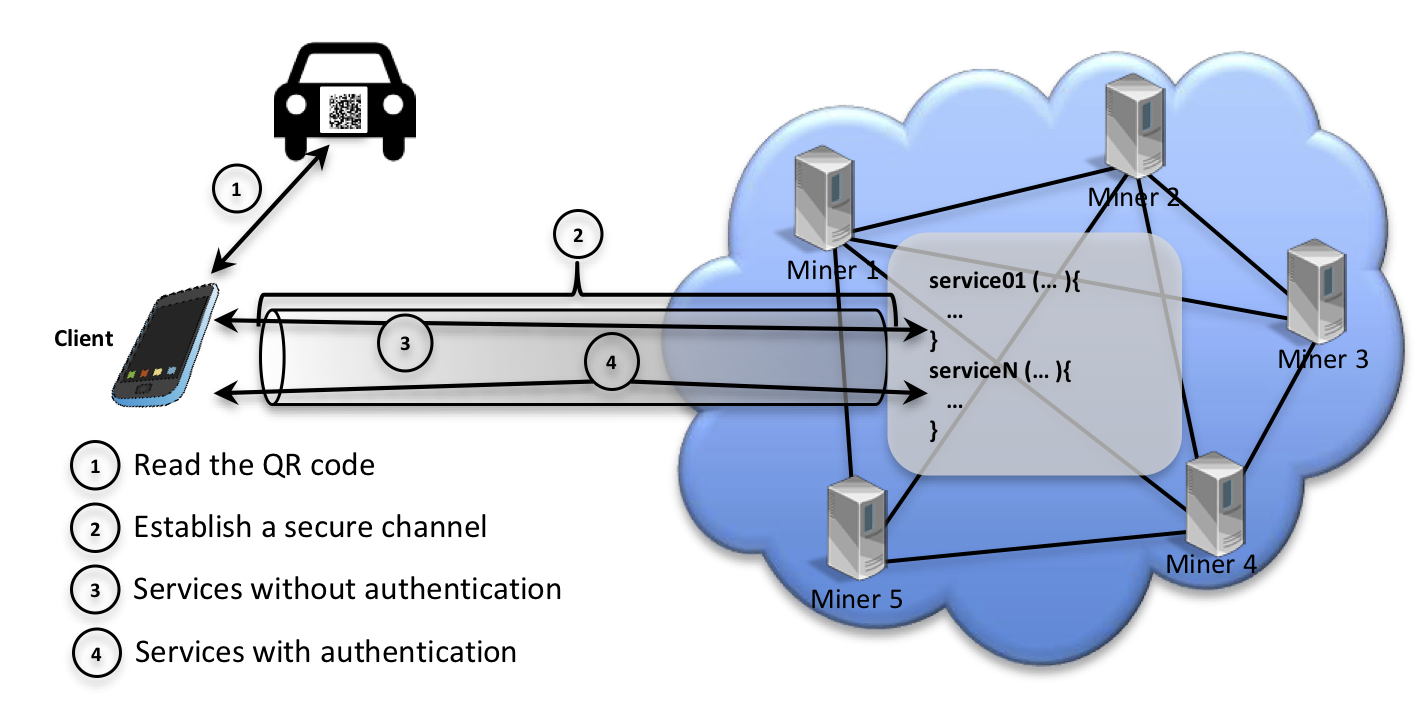
\includegraphics[scale=0.74]{images/lopez2.png}
        \caption{Diagram about the use of the framework from the client view}
    \label{fig:flowChartFramework}
 % \end{center}
\end{figure}

\begin{itemize}
  \item \textbf{Stage I} consists in getting information of a vehicle through reading
    a QR code by any user.
    %or setting the QR code by a dealership. 
    This stage requires that a company generates the genesis block after a vehicle has 
    been manufactured. Details in Section~\ref{ssec:clientServer}.
  \item \textbf{Stage II} consists in establishing a secure channel between any user
    and the \textit{vehicle blockchain network}. We
    have used the TLS protocol because it is the standard in the
    e-commerce and it has been subject to a lot of verification proofs.
    Details in Section~\ref{sec:secureChannel}.
  \item \textbf{Stage III} consists in getting services such as provenance or 
    traceability. Some services require authentication, but others do not.
    Details in Section~\ref{sec:getServices}.  
  \item \textbf{Stage IV:} consists in how to do transactions and what kind of these can 
    do each role (owner, government, dealerships, etc). For example how to build
    the genesis block within the \textit{vehicle blockchain network}. 
    Authentication is required. 
    Details in Section~\ref{sec:transactions}. 
\end{itemize}

\subsection{Notation}
\label{sec:notation}
%As you can see, our stages imply the use of cryptography,  and security protocol techniques. 
% The following two sub-sections describe the notation used in the rest of
% the document. 

% \subsubsection{Host level notation}
% \label{sec:hostLevel}
Our notation has some similarities with Burrows et.al.~\cite{Burrows1990}. 
Table~\ref{table:conventions} summarizes our notation. Let start with
cryptography, it has two main mechanisms:
\begin{itemize}
  \item Symmetric cryptography, the same key is used to encode and
    decode a message; by convention, symbol $\fat{m}_{K_{AB}}$ will be
    used to denote that a message $m$ has been cyphered under the key
    $K_{AB}$, which agents $A$ and $B$ know. \footnote{An agent is a 
        computer process that uses the client-server technology to 
        establish a network communication. Sometimes we will use the 
        terms agent or client indistinctly.} 
  \item Asymmetric cryptography, two keys are used to encode and
    decode messages; an agent (e.g. $A$) has a key pair
    (public $K_{pub(A)}$ and private $K_{priv(A)}$). One key used to
    encode and the other one to decode (reciprocally); usually, key
    $K_{priv(A)}$ is kept in secret. 
\end{itemize}

\begin{table}[htb]
\footnotesize
\begin{center}
\caption{Conventions in types of messages and agents}
\label{table:conventions}
\begin{tabular}{|l|l|}
\hline
{\bf Abbreviation}& {\bf Description}                                   \\\hline\hline
$C$                 &  Agent, Client or Smartphone application able to \\
                    &  establish communication with other agent.         \\ 
$\Server$           &  A trusted agent, best known as trusted Miner-Server      \\
$K$                 &  Symmetric key                                      \\
$K_{AB}$            &  Symmetric key shared with agents $A$ and $B$       \\
$K_{pub(A)}$        &  Public key of Agent $A$                            \\
$K_{priv(A)}$       &  Private key of Agent $A$                           \\
$\fat{m}_{K}$       &  Message $m$ cyphered under key $K$                 \\
$m1\lnk m2$         &  $m1$ and $m2$ are concatenated using symbol $\lnk$ \\
$[m_1:: m_2]$       &  A list o messages, $m_1$ representing the first element\\
$N_a$, $N_b$, $N_c$ &  Nonces, which are random unguessable numbers      \\
                    &  never been used before.                           \\ \hline \hline
\end{tabular}
\end{center}
\end{table}
\normalsize

% \subsubsection{Notation at network level}
% \label{sec:networkLevel}
Table~\ref{table:NetConventions} describes the notation in the Client-Server communication.
Our model is compound by various security protocols. A security protocol is formed by the 
initial knowledge of the participant agents and a set of message steps. Each step consists in  
sending or receiving messages under the Client-Server technology. Before sending a message,
an agent can execute an operation (maybe dependent of the previous received message), as part 
of a local process.

%three views (see ): i) initial knowledge;
%ii) message sending and message reception; and iii) the local process
%representation.
\begin{table}[htb]
\footnotesize
\begin{center}
\caption{Conventions in network level}
\label{table:NetConventions}
\begin{tabular}{|l|l|}
\hline
{\bf Abbreviation}                      & {\bf Description}                    \\\hline\hline
\textbf{Initial knowledge:}             &                                      \\
$A : ik$                                &  Initially agent $A$ knows $ik$.    \\ \hline 
\textbf{Message Sending and Receiving:} &  At step $n$ agent $A$ sends         \\ 
$n. A \rightarrow B: m$                 &  message $m$ to agent $B$,\\
                                        &  which $B$ receives.      \\ \hline 
$n. A\rightarrow B: m$                  &  message $m2$ was generated \\ 
\hspace{5mm}\textbf{Local process:}     &  Between steps $n$ and $n2$,    \\ 
\hspace{5mm}$m2 = f(m)$                 &  by $B$ as a local process \\ 
$n2. B\rightarrow A: m2$                &  generated from $f(m)$.     \\ \hline 
\textbf{Broadcast:}                     &  $A$ broadcasts message to agents\\ 
$A \rightarrow [B, C, D]: m$            &  $B$, $C$ and $D$.\\ \hline \hline 
\end{tabular}
\end{center}
\end{table}
\normalsize


$$$$


 %added by JC        
        \section{Secure communication between agents}
\label{sec:client}
This section describes mainly two parts: 
a) who are the participant agents, the QR code generation and by whom; and 
b) after having read the QR code, how the communication between the agents are securely 
carried out using the TLS protocol.

\subsection{Client-Server Participants and the QR Code}
\label{ssec:clientServer}
QR code can be read quickly by many modern cell phones. It is used to take a piece of 
information from a transitory media and put it in to your cell phone. 
It may give you details about a URL, vCard, plain text, etc.

Our solution takes into account an application able to read a QR code (i.e. an smartphone).
The application must be able to connect with the \blockchaincarnetwork in order
to do different operations (Table~\ref{table:operations} shows a list of operations). 

In particular, the smartphone application is denoted as the client $\Client$. 
It, while requesting communication, connects with a miner, denoted as \Server, within the set of the \blockchaincarnetwork.


%\subsubsection{Setting a QR Code in a Car}
%\label{sssec:settingQR}
The QR code must be generated by dealerships who manufactures vehicles and they must place the code
in both: physically in some part of the vehicle and virtually in the invoice.

Let the QR code content the following data: 
\textit{id=vehicle identification number}, 
\textit{trademark}, 
\textit{model}, 
\textit{class}, 
\textit{version}, 
\textit{number of cylinders}, and
among \textit{others}. These attributes are own of a vehicle, and they do not 
change with time. An example in JSON format is shown in Table~\ref{table:genesisInfo}.
The QR code information is formated in plain-text because such an information is not sensitive and anyone can obtain it.
\begin{table}[h]
    \centering
    \caption{Genesis information about the vehicle}
    \begin{tabular}{lll}
       \{&         			&    							\\
         & id:        		& "1FMYU02Z97KA580G2", 			\\
         & tradeMark: 		& "abcd", 						\\
         & model:     		& "2012", 						\\
         & class:     		& "auto", 						\\
         & version:   		& "TA XLS 4X2 I4 TELA 4 CIL", 	\\
         & cylinders: 		& "L4" 							\\
       \}& 		        	& 								\\
       ::& \textit{others}	&								\\
    \end{tabular}
    \label{table:genesisInfo}
\end{table}


%\subsubsection{Client-Server Parts}
%\label{sssec:readingQR}



%Throughout this document, we refer to \QR code as the information obtained after a reading 
%process. 

\subsection{Establishing a secure channel}
\label{sec:secureChannel}
Messages transmitted on the Internet are sensitive to be seen for
active or passive attackers who are able to manipulate them in order
to take advantage of the situation.

Transport Layer Security (TLS) and its predecessor, Secure Socket
Layer (SSL), is a \emph{cryptographic protocol} that works over the transport 
layer of the Internet Protocol (TCP/IP model). This protocol allows client/server 
agents to communicate securely by tunnelling a hostile network like Internet. 

%We have used the TLS protocol because, besides being the 
%standard in e-commerce, the identity of the client is not
%relevant while consulting information. 
%However, for transactions that 
%require authentication, then we have taken an additional step that we will 
%explain later.

Table~\ref{table:sslAndtlsProtocol} shows the protocol in Alice and Bob 
notation, it has been adapted from \cite{lopez13} and its explanation is as follows:
\begin{table}[htb]
\footnotesize
\begin{center}
\caption{SSL and TLS Protocol}
\label{table:sslAndtlsProtocol}
\begin{tabular}{|l|}
\hline
  Initial Knowledge                                                                     \\\hline
            $C:C\lnk QR$                                                                  \\ 
            $\Server: K_{pub(S)}\lnk K_{priv(S)} \lnk \Server$                 \\ 
            $\Servera: \forall K_{pub}\in \Key$                                   \\ \hline 
  Generating a session secret key                                                          \\
            1.-$\Client\rightarrow \Server:C\lnk N_{C}\lnk [Lc]$                         \\ 
            2.-$\Server\rightarrow \Client: f([Lc])\lnk \Server \lnk N_{\serverW}\lnk N_{C}\lnk 
                 K_{pub(\serverW)}\lnk S_{ca}\lnk $                                            \\ 
            \hspace{3mm} $\fat{Hash(\Server\lnk N_{\serverW}\lnk N_{C}\lnk K_{pub(\serverW)}\lnk 
                        S_{ca})}_{K_{priv(\serverW)}}$                                          \\ 
            3.-$\Client\rightarrow \Servera:$verification process with $\Servera$             \\ 
            4.-$\Servera \rightarrow \Client: \Server$ is authenticated                     \\ 
            5.-$\Client\rightarrow \Server: N_{C}\lnk\fat{C\lnk N_{C'}}_{K_{pub(\serverW)}}$      \\ \hline
  New knowledge accumulated                                                               \\
            $C:C\lnk QR \lnk N_{C}\lnk K_{pub(\serverW)}\lnk N_{C'} \lnk $                                    \\
            \hspace{5mm} $K_{\client\serverW}=Hash(N_{C'},N_{C},N_{\serverW})$                              \\ 
            $\Server: K_{pub(\serverW)}\lnk K_{priv(\serverW)}\lnk \Server\lnk N_{C}\lnk N_{C'}\lnk$    \\
            \hspace{5mm} $K_{\client\serverW}=Hash(N_{C'},N_{C},N_{\serverW})$                               \\ \hline
            \textbf{Security Properties}                        \\
            \hspace{5mm}Secrecy of $K_{\client\serverW}$ known by $[\Client,\Server]$ \\
            \hspace{5mm} $\Client$ authenticates $\Server$ on $K_{\client\serverW}$        \\
            \hline \hline            
            \hline 
\end{tabular}
\end{center}
\end{table}
\normalsize

\begin{itemize}
  \item Initially, $\Server$ denotes a trusted miner server. $\Client$ denotes
    a user having read a QR code, and $\Servera$ denotes a server certification 
    authority. $\Server$ knows its public and private key; all (client and servers) 
    know their own identities. $\Servera$ knows all issued
    public keys. Here $\Key$ denotes a set of all public keys.
  \item Then, the following steps are carried out in order to
    establish the secure tunneling:
    \begin{itemize}
    \item \textbf{First step:} a client connects to a TLS server
      requesting a secure connection (in plain-text) and presents a list
      of supported CipherSuites (ciphers and hash functions),
      $[Lc]$. Each session is identified by a session id $N_{C}$. 
    \item \textbf{Second step:} from list, the server picks the
      strongest cipher and hash function that it also supports
      ($f([Lc])$) and notifies the client of the decision. The server
      sends back its identity in the form of a digital certificate and
      in plain-text. The certificate and the plain-text usually contains
      the server name $\Server$, the server's public encryption
      key and the trusted certificate authority $\Servera$. 
    \item \textbf{Third step:} the client may contact the
      server that issued the certificate and confirms that the
      certificate is valid before proceeding.
    \item \textbf{Forth step:} the certification authority sends back to the 
      client a confirmation about the credibility of the key.
    \item \textbf{Fifth step:} in order to generate the session keys used for the
      secure connection, the client encrypts a nonce number $N_{C'}$
      with the server's public key and sends the result to the
      server. Only the server should be able to decrypt it, using its
      private key.  
    \end{itemize}
\item Finally, from the nonce numbers $N_{\client}$, $N_{\client'}$ and $N_{\serverW}$
    the session key, $K_{\client\serverW}$, is generated and will be used  in the 
    following transactions for encryption and decryption operations.   
    In the TLS protocol only the server is authenticated ($\Client$ \textit{authenticates} $\Server$ on $K_{\Client\Server}$), but not vice-versa.
    The new session key generated between $\Client$ and $\Server$ is kept in secret, but $\Server$ cannot be safe about $\Client$ identity.
    Hence, an authentication step is required, see Section~\ref{ssec:SecAuth}.
\end{itemize}



 %added by JC        
        \section{Get services}
\label{sec:getServices}
Figure~\ref{fig:dfdForAuthServices} illustrates a Data Flow Diagram (DFD) about consuming  
services and set transactions. The Figure shows the scenarios when authentication is or 
not required. Independently of that, the secure channel (described in Section~\ref{sec:secureChannel}) 
is required.

\begin{figure}[hb]
 %\begin{center}
  \centering
    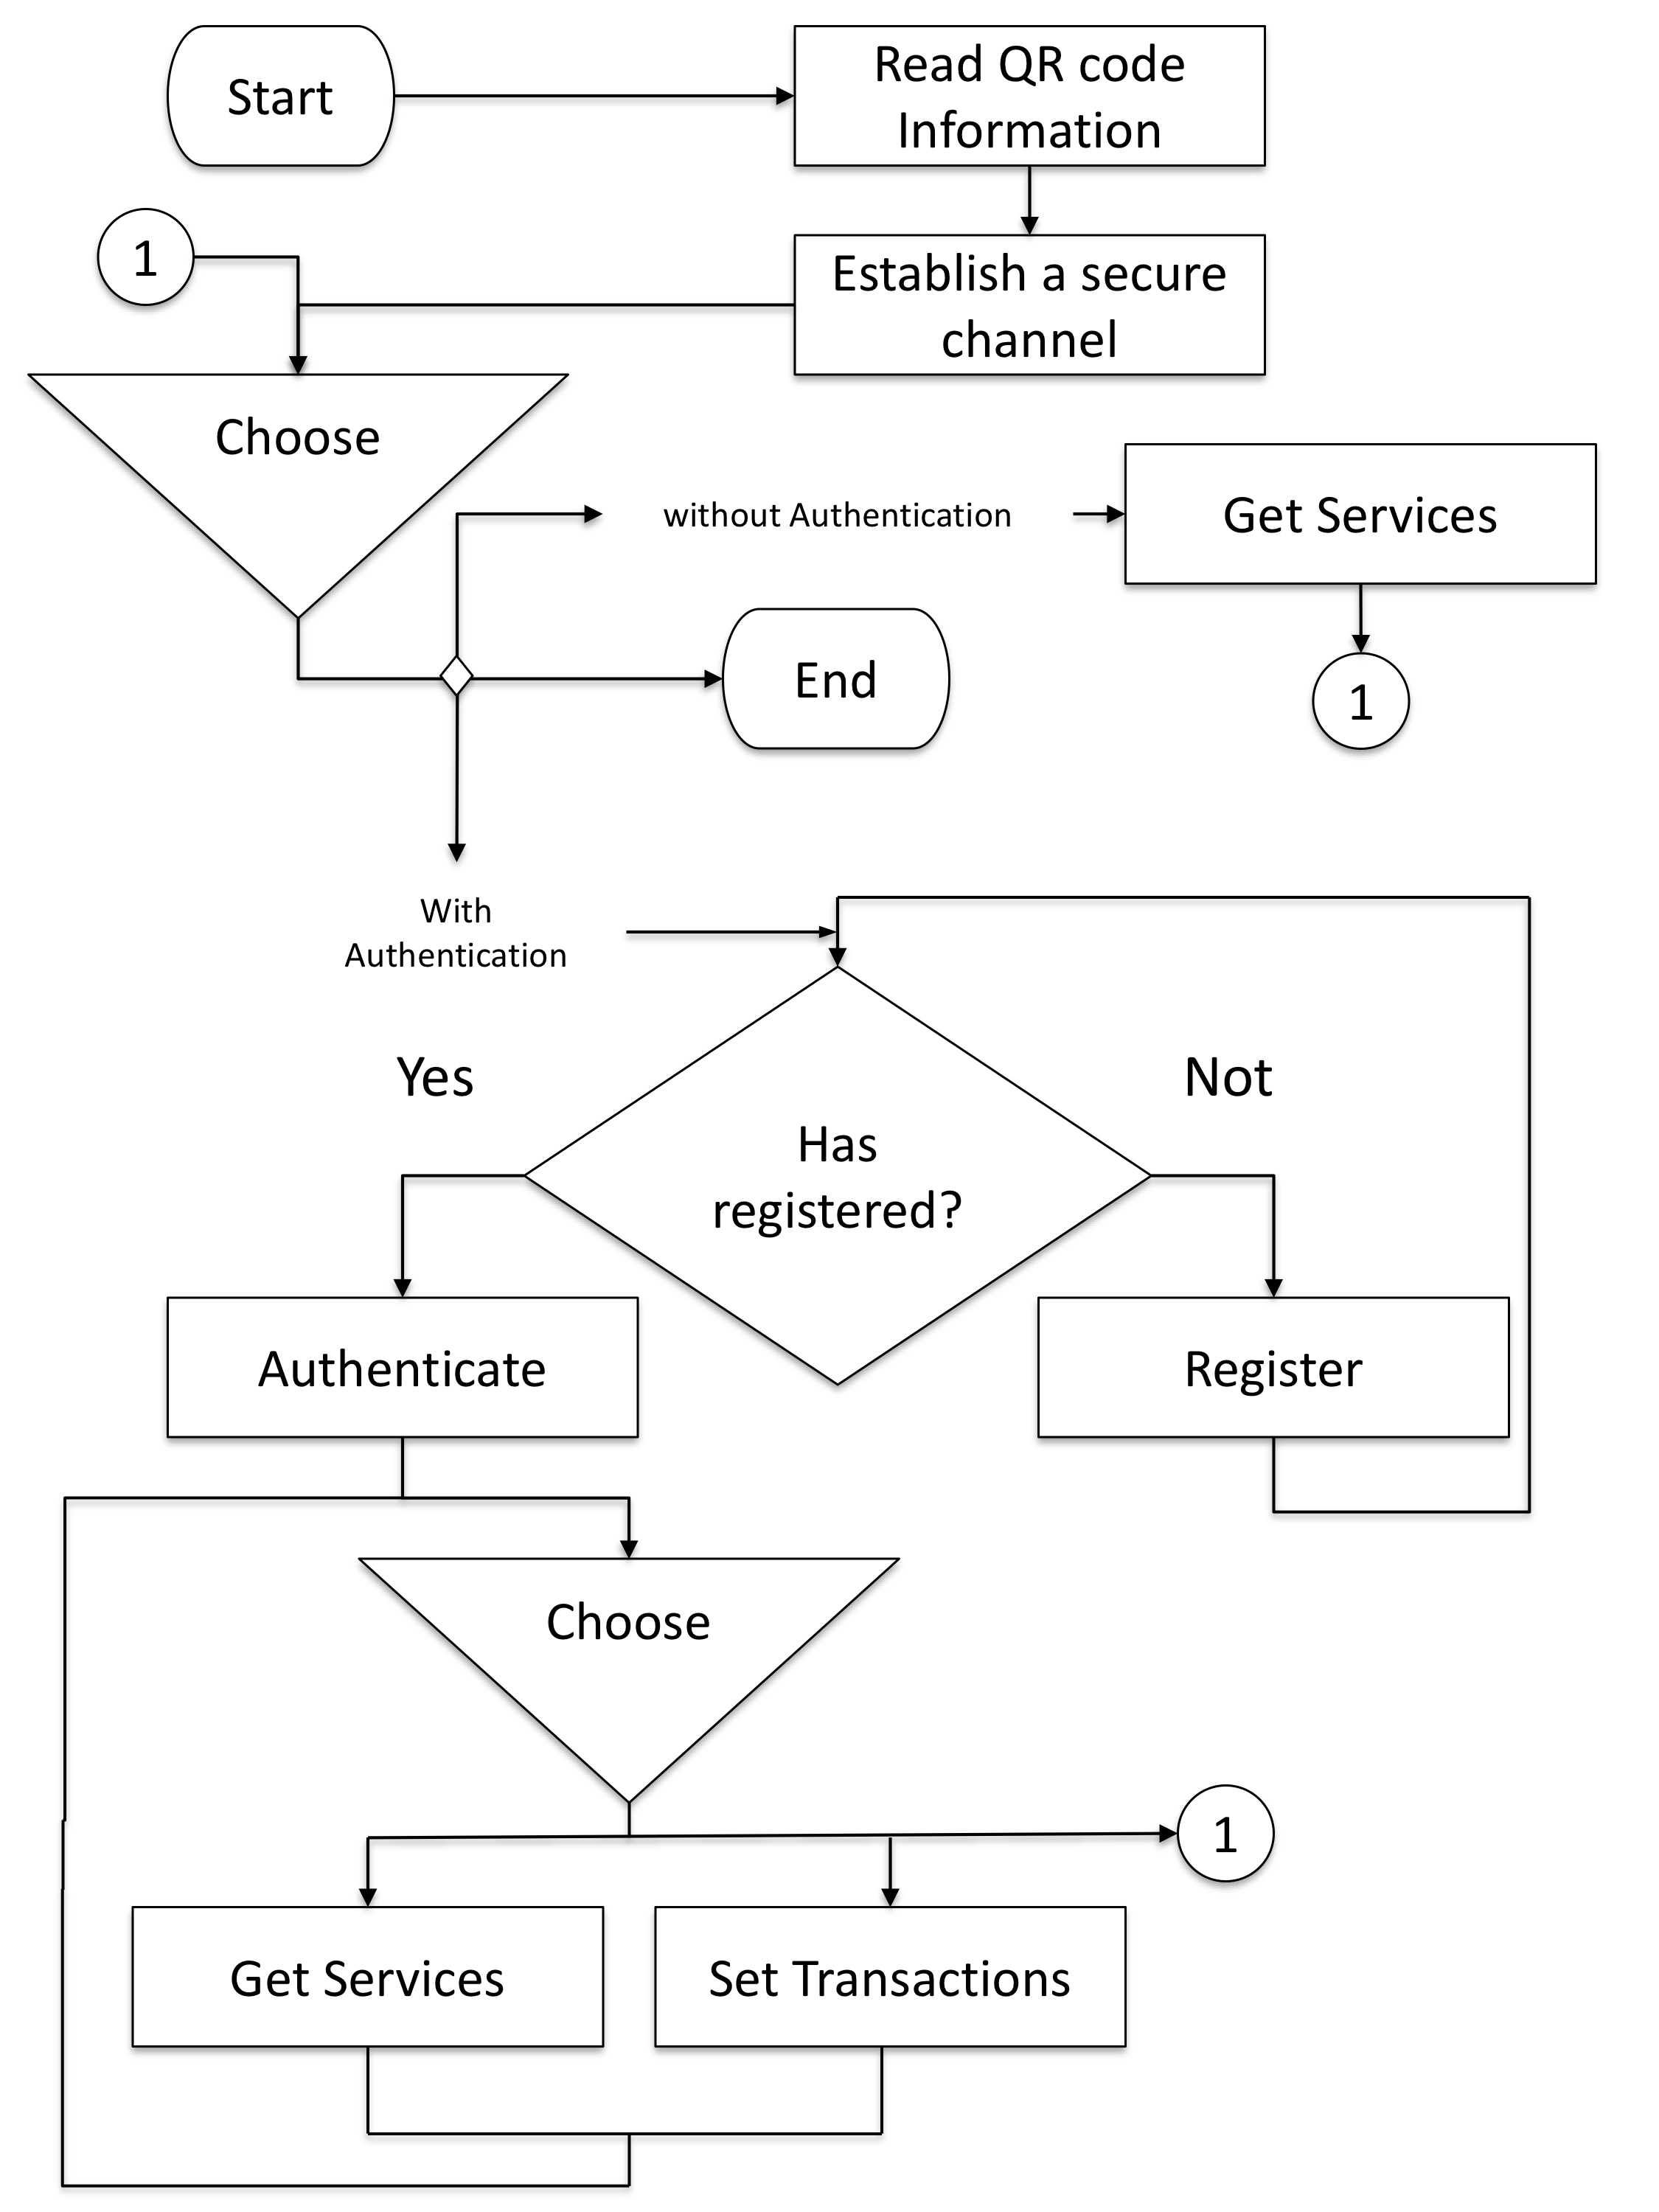
\includegraphics[scale=0.35]{images/lopez3.png}
        \caption{General DFD about consuming services and set transactions}
    \label{fig:dfdForAuthServices}
 % \end{center}
\end{figure}

\begin{table}[htb]
\footnotesize
    \begin{center}
    \caption{Services, require or nor authentication }
    \label{table:servicesPermits}
        \begin{tabular}{l|l|l|l}
			\textbf{Num.}&\textbf{Service}		 &Yes    &Not    \\ \hline
             1			 &Theft status           &       &X      \\ \hline
             2			 &Debt status            &       &X       \\ \hline
             3			 &Basic characteristics  &       &X       \\ \hline
             4			 &Owners                 &X      &       \\ \hline
             5			 &Arrested history       &X      &       \\ \hline
             6			 &Penalties history      &X      &       \\ \hline
             7			 &Tax history            &X      &       \\ \hline
        \end{tabular}
    \end{center}
\end{table}


\subsection{Getting services without authentication}
\label{ssec:getServNoAuth}
Some services must be available for all users and without the need to be 
authenticated 
(Table~\ref{table:servicesPermits} defines what services require or not authentication), 
achieving thus transparency. 
For example, to know:
\begin{itemize}
    \item If a vehicle hold currently a theft or debt report.
    %\item If a vehicle hold currently a debt report.
    \item Some basic characteristics such as \textit{trademark}, \textit{model}, 
        \textit{class}, \textit{version} and \textit{cylinders}.
\end{itemize}


%The network connection starts when a user $C$ contacts to the \blockchaincarnetwork~ 
%through miner $\Server$. 
Table~\ref{table:ProtGetServicesNoAuth} describes how to get services without authentication,
the explanation is as follows:
\begin{itemize}
  \item  The initial knowledge consists in all values learned by the client, $C$, and the 
    \blockchaincarnetwork~ $\Server$ after completed the secure channel stage 
    (described in Section~\ref{sec:secureChannel}).
   \item The request of a service consists in sending an identity $C$, the data of the $QR$ code, and a 
        number $n$ denoting the number of service that is requested to be consumed. 
        The client ciphers  these messages using the secret key $K_{C\Server}$ obtained in
        the secure channel stage. 
        %(see Section~\ref{sec:secureChannel}).
   \item The miner $\Server$ (having a copy of all blockchains within the \blockchaincarnetwork) verifies 
        if such a service can be consumed (according permissions) and then, 
        returns the answer $d$; ciphered using, again, the shared secret key $K_{C\Server}$. Finally,
        $C$ decodes the message and shows the information $d$ to the user.
\end{itemize}


\begin{table}[htb]
\footnotesize
\begin{center}
\caption{Get Service Protocol, authentication is not required}
\label{table:ProtGetServicesNoAuth}
\begin{tabular}{|l|}
\hline
           Initial Knowledge                                                             \\
            $C:C\lnk QR \lnk  K_{\client\serverW}$                                    \\
            $\Server: \Server\lnk K_{\client\serverW}$    \\ \hline \hline 
           Get a service                                                                        \\
           1.-$\Client\rightarrow \Server: \fat{C \lnk QR \lnk n}_{K_{\client\serverW}}$          \\ 
           \hspace{5mm} $d=getService(QR,n)$                                  \\  
           2.-$\Server\rightarrow \Client: \fat{C \lnk d}_{K_{\client\serverW}}$       \\ \\ \hline \hline
\end{tabular}
\end{center}
\end{table}
\normalsize


\subsection{Get Services with authentication}
\label{ssec:ServAuth}
Sometimes it will be necessary to know who is consuming some services; or maybe the service consumes extra 
computational power. For that, client and miner must be authenticated. 

Transport Layer Security (TLS) allows client/server agents to communicate 
across a hostile network, but eventually, only the server is authenticated. 
Mutual authentication requires a public key infrastructure for clients, which
we achieve by mean a \textit{registration process}. 

\subsubsection{Registration with the Blockchain vehicle wallet}
\label{sec:Registration}

This part consists in to establish a \textit{username} and a \textit{password}, which
will be mapped with an identity. The \textit{username} must be a valid email and the 
\textit{password} will be created by the user.

Table~\ref{table:reqSessKey} summarizes the protocol
in Alice\&Bob notation, its description is as follows: 
\begin{itemize}
  \item Firstly, the user must establish a secure channel with the miner-vehicle-wallet\footnote{
    We will use server-wallet to abbreviate miner-vehicle-wallet.},
    $K_{C\ServerW}$,
    (see Section~\ref{sec:secureChannel}). In this step all exchanged messages are ciphered 
    using the symmetric key $K_{C\ServerW}$, which was obtained during the TLS protocol. 
  \item Secondly, the user must generate his key pair (public and private) through
    his username and password executing the following steps:
    \begin{itemize}
    \item \textbf{First step:} the client sends his username denoted with his email $@$, and  
        a list of personal data $Pd$. 
    \item \textbf{Second step:} the server-wallet sends back the user via an email server $\Client_e$ a 
        data obtained of the client's personal information, $Pd$ and a challenge $X=f(Pd)$. 
    \item \textbf{Third step:} then, the client must generate the final password $P$, but
      only the hash is sent, $Hash(P,X)$.  Sending $Hash(P,X)$, we can
      ensure that $P$ will be only known by $\Client$.
    \item \textbf{Fourth step:} the miner-wallet creates a public and private key for the client 
        ($K_{pub(\Client)}$ and $K_{priv(\Client)}$), which the system maps with the client and 
        the hashed password; builds a block $bp$ containing the public key of the client and broadcasts
        it to the \blockchaincarnetwork to do the mining process. 
    \item \textbf{Fifth step:} After the mining process, the miner-wallet provides to the $\Client$ the 
        public and private key; which will be used to do transactions. 
    \end{itemize}
\end{itemize}
Note that, any user could transact a lot of accounts with the miner-wallet, but each of their 
vehicle-wallet would be empty.

\begin{table}[htb]
\footnotesize
\begin{center}
\caption{Client registration process}
\label{table:reqSessKey}
\begin{tabular}{|l|}
\hline
%{\bf Process}                                                                \\\hline\hline
%Initial Knowledge                                                             \\
%$C:N_{C}\lnk K_{pub(S)}\lnk N'_{C} \lnk K'_{CS}$                              \\
%$\ServerW: K_{pub(S)}\lnk K_{priv(S)}\lnk \ServerW\lnk N_{C}\lnk N_{C'}\lnk 
%                      K'_{CS}$                                                \\ \hline \hline
Initial Knowledge                                                             \\
$\Client:K_{C\ServerW}\lnk [@::Pd]$                                                    \\
$\ServerW: K_{C\ServerW}$                                                            \\ \hline \hline
1.-$\Client\rightarrow \ServerW:\fat{[@::Pd]}_{K_{\Client\ServerW}}$                     \\
\hspace{5mm} $X=f(Pd) $                           \\ 
2.-$\ServerW\rightarrow \Client_e: \fat{@\lnk Pd \lnk X}_{K_{\Client_e\ServerW}} $                  \\ 
\hspace{5mm} $\Client$ generates password $P$                          \\  
3.-$\Client\rightarrow \ServerW:\fat{@\lnk Hash(P,X)}_{K_{\Client\ServerW}}$                 \\  
\hspace{5mm} $\ServerW$ generates a pair key ($K_{pub(\Client)}$ and $K_{priv(\Client)}$)\\
\hspace{5mm} $\ServerW$ generates a block $bp = blockPubKey(K_{pub(\Client)})$\\
4.-$\ServerW\rightarrow [\Server_i .. \Server_n]: \fat{\ServerW \lnk bp}_{K_{\Server_i .. \Server_n}}$  \\  
5.-$\ServerW\rightarrow \Client: \fat{C \lnk K_{pub(\Client)}\lnk K_{priv(\Client)}}_{K_{\Server}}$          \\            \hline
New Knowledge Accumulated                                                     \\
$\Client:P\lnk X \lnk K_{pub(\Client)}\lnk K_{priv(\Client)}$                                                                \\
$\ServerW: K_{pub(\Client)}\lnk K_{priv(\Client)}\lnk X \lnk Hash(P,X)\lnk [@::Pd]$       \\\hline \hline 
\end{tabular}
\end{center}
\end{table}
\normalsize




The security properties the protocol must provides are: $P$ to be
known only by $C$; $K_{pub(\Client)}$ and $K_{priv(\Client)}$ to be known by $\Server$; 
and obtain strong authentication between the participants.

% We have verified this protocol using The AVISPA Tool Web
% Interface, available via http://www.avispa-project.org/
% finding the following:
% \begin{itemize}
%     \item The protocol provides secrecy.
%     \item We have proved that the protocol provides
%       \emph{authentication} from the client to the server on message 
%       $f(Pd)$ and \emph{weak authentication} from the server to the
%       client on message $Hash(P)$.
%     \item When we proved \emph{strong authentication}, it failed due
%       to the lack of freshness property generating The Dolev and Yao
%       attacker (of AVISPA tool) a replay attack. However, this attack
%       is already not possible when we consider that $K'_{CS}$ is
%       fresh, which was obtained in an immediately previous step. Even
%       though, we could include timestamps in all steps, however, that
%       is not necessary. 
% \end{itemize}

\subsubsection{Client-Miner Authentication}
\label{ssec:SecAuth}


The authentication process trusts in the users' \textit{username} 
(email) and \textit{password}, so, it is responsibility for the user 
to ensure his secrets. However, it is well known that any system 
cannot trust only in a user and password control access, because of that, 
it is important not only to encrypt the sensible information, but also
to implement more security mechanisms (like authentication procedure) to 
avoid possible attacks.

The goal of this stage is to establish authentication between a client and 
a miner after having a secure tunneling. Note that, public and private key
of the user are not used for the authentication process, it is only used to
do transactions. Table~\ref{table:AuthProtocol} 
describes the authentication part and the explanation is as follows:

\begin{itemize}
  \item Both the client and the miner store all knowledge accumulated
    of previous steps. It is considered to have established a secure tunneling 
    with the miner using the TLS protocol and to have obtained the register
    procedure. So, the initial knowledge of the client consists in to know 
    the session key $K_{\Client\Server}$, his password $P$ and the secret $X$. 
    On the other hand, the miner knows the same session key, the client public and
    private key, personal information of the client, secret $X$ and the hashed 
    $Hash(P,X)$. The following steps are proposed:
    \begin{itemize}
    \item \textbf{First step:} the client sends a challenge to the
      miner $N_\Client$. The miner can map $@$ with $\Client$ and build $hash(@\lnk\Client\Server\lnk N_\Client)$. This message is ciphered with $K_{\Client\Server}$ because the session key has been destined for them. 
    \item \textbf{Second step:} the server responds to the client with a new challenge,
      firstly includes the client name $C$ (which is mapped with $@$) and a hashed message
      $Y$ composed by $N_{\Client}$ and $X$ both messages must be known by the client. Again,
      all ciphered with $K_{\Client\Server}$.
    \item \textbf{Third step:} Once the client has accepted the previous step, it means that
      he has deduced all previous messages and he has authenticated to the miner, so, the 
      client sends back his username $@$, the challenge response $N_\Client$ as a freshness
      property and his password concatenated with $P$, $X$ and $N_{\Client}$.
  \end{itemize}
\item Finally, after having run the protocol it is expected to obtain strong authentication
    between the client and the miner. 
\end{itemize}
 
\begin{table}[htb]
\footnotesize
\begin{center}
\caption{Authentication Protocol}
\label{table:AuthProtocol}
\begin{tabular}{|l|l|l|}
\hline
{\bf Process}                                                                     \\\hline\hline
            Initial Knowledge                                                     \\
            $\Client:P\lnk X \lnk K_{\Client\Server}$                               \\
            \hspace{5mm}                                                 \\ 
            $\Server: K_{pub(\Client)}\lnk Hash(P,X)\lnk X \lnk[@::Pd] \lnk K_{\Client\Server}$ \\\hline \hline
            Authentication                                                         \\
            1.-$\Client\rightarrow \Server: \fat{\Server \lnk @ \lnk N_{\Client} \lnk 
                                              Hash(@\lnk \Client \lnk \Server \lnk N_\Client)}_{K_{\Client\Server}}$  \\ 
            2.-$\Server\rightarrow \Client: \fat{\Client \lnk hash(N_{\Client},X)}_{K_{\Client\Server}}$ \\ 
            \hspace{5mm} $Y=hash(N_{\Client},hash(P,X))$                          \\              
            3.-$\Client\rightarrow \Server: \fat{@\lnk N_{\Client}\lnk Y}_{K_{\Client\Server}}$            \\ \hline  \hline
            New Knowledge Accumulated                                               \\
            $\Client: \Server \lnk N_\Client \lnk Y$         \\
            \hspace{5mm}                \\ 
            $\Server: \Client  \lnk N_\Client \lnk Y$          \\ 
            \hspace{5mm}                             \\ \hline \hline
\end{tabular}
\end{center}
\end{table}
\normalsize



\subsubsection{Get Services with authentication}
\label{ssec:getServAuth}
Some services are available only after the authentication process, for example, to know:
\begin{itemize}
    \item A history of owners
    \item How many times the vehicle has been arrested 
    \item The number of penalties
    \item A history of taxes.
\end{itemize}

See Table~\ref{table:servicesPermits} to identify what services require authentication.
Table~\ref{table:ProtGetServicesAuth} describes in Alice and Bob notation how to get services 
requiring an authentication process, the explanation is similar to that in 
Section~\ref{ssec:getServNoAuth}, next we explain the differences. 

As you can see, the difference with respects to 
Table~\ref{table:ProtGetServicesNoAuth}, where authentication is not required, is that in steps
1 and 2, the hashed message $Y$ is include.

Here, after step 1, the miner verifies if such a service can be consumed (according permissions, see
Table~\ref{table:servicesPermits}) and then, returns the answer $d$; in a ciphered way as above was 
explained.






\begin{table}[htb]
\footnotesize
\begin{center}
\caption{Get Service Protocol with authentication}
\label{table:ProtGetServicesAuth}
\begin{tabular}{|l|}
\hline
           Initial Knowledge                                                             \\
            $C:C\lnk QR \lnk  K_{\client\serverW} \lnk Y$                                    \\
            $\Server: \Server\lnk K_{\client\serverW} \lnk Y$    \\ \hline \hline 
           1.-$\Client\rightarrow \Server: \fat{C \lnk QR \lnk n \lnk Y}_{K_{\client\serverW}}$          \\ 
           \textbf{Get a service}                                                                        \\
           \hspace{5mm} $d=getService(QR,n)$                                  \\  
           2.-$\Server\rightarrow \Client: \fat{C \lnk d \lnk Y}_{K_{\client\serverW}}$       \\ \\   \hline \hline
\end{tabular}
\end{center}
\end{table}
\normalsize





 %added by JC  ---
        \section{Transactions}
\label{sec:transactions}
A transaction is an exchange or transfer of goods, services, or funds where it can involve 
two parties or things that reciprocally affect or influence each other. 
As shown in Table~\ref{table:operations} the operations are involved in at least two parts (\textit{sell} and \textit{buy}, for instance). These parts are different roles that a client can 
acts at different moments.



\subsection{Roles}

According to the permissions the users will have five defined roles: 
\textbf{U}ser,
\textbf{D}ealership,
\textbf{O}wner,
\textbf{G}overnment, and
\textbf{H}elper.
Each user could hold one or more roles.
Table \ref{table:operations} pinpoints the type of operations that each role can do and the explanation
is as follows: 
\begin{itemize}
    \item Any \textbf{U}ser will have enough permissions to interact with the system in order to 
        obtain information on the vehicle (Section~\ref{sec:getServices}). This role is also able 
        to buy cars, but it must be authenticated. 
        These permissions will be granted to the user once he has established the secure channel. 
    \item The \textbf{D}ealership is able to manufacture vehicles because of that he is who creates the 
        genesis block.
    \item Every car will have one and only one \textbf{O}wner at a given time. The owner will be the only one 
        that has permission to trade ownership, but also to request to the government to change legal
        status. In addition, he can request and authorize to \textbf{H}elper to add some information 
        about a car.
    \item \textbf{G}overnment will have the ability to  \textit{change legal status} when the 
        vehicle is involved in legal situations. For that, it will be necessary to establish 
        different status: \textit{stolen}, \textit{arrested}, \textit{penalty}, \textit{registered owner}, \textit{plate}, 
        \textit{tax history}, etc.
    \item The \textbf{H}elper role is who receives a temporal permission from the \textbf{O}wner to set one 
        transaction on the block-chain. The time frame for the temporal permission will be authorized by 
        the \textbf{O}wner of the car. The car owner will set a special transaction to give the helper 
        the permission. The helper role will be used for transactions that change one or more data of the 
        car's properties. This will include official services, mechanical adjustments, big aesthetic 
        modifications and insurance payments.
\end{itemize}

Each user, acting with a different role, is forced to execute a transaction and to fulfill a contract.
Since, transaction histories are becoming more transparent and secure through the use of blockchain 
technology. All network participants share the same information (through blocks) as opposed to 
individual copies. To modify a single transaction record would require the alteration of all subsequent 
records and the collusion of the entire network.




\begin{table}[htb]
\footnotesize
    \begin{center}
    \caption{Type of operation grouped by corresponding transactions}
    \label{table:operations}
        \begin{tabular}{|l|l|l|l|l|l|}
        \hline
        \textbf{Operation}          &\textbf{U}& \textbf{D}&\textbf{O}& \textbf{G}& \textbf{H}\\ \hline\hline
        Create (genesis block)      &          & X         &          &           &           \\ \hline\hline
        get information             & X        &           &          &           &           \\ \hline\hline
        sell                        &          &           & X        &           &           \\ \hline
        buy                         & X        &           &          &           &           \\ \hline\hline
        request change legal status &          &           & X        &           &           \\ \hline
        change legal status         &          &           &          & X         &           \\ \hline\hline
        request to add information  &          &           & X        &           &           \\ \hline
        add information             &          &           &          &           & X         \\ \hline
        authorize add information   &          &           & X        &           &           \\ \hline
        \end{tabular}
    \end{center}
\end{table} %added by JC


\subsection{Set Transactions} 
\label{ssec:setTrans}
As shown by Table~\ref{table:ProtSetTrans} the participants in a transaction 
are a client (acting any role, sometimes like \textbf{O}wner or \textbf{D}ealership, etc) and a miner.
The client knows the $QR$ code through a scan process with
a car; a secret shared key $K_{\client\serverW}$ established with
a miner in the secure channel process; a proof to have been authenticated
with the miner $N_{\client\serverW}$; and the transaction $T$ that client wish 
to do  (see Table~\ref{table:operations} for types of operations). 
The miner obviously knows also $K_{\client\serverW}$ and $N_{\client\serverW}$. 
\begin{enumerate}
    \item The protocol starts when the client $\client$ builds the transaction 
        data $t$, the signature of the transaction $\fat{t}_{K_{priv(\client)}}$ and sends
        all to the miner $\Server$; all ciphered with the 
        session key $K_{\client\serverW}$. 
    \item Having the miner accepted the previous message (verifying the  
        session with $N_{\client\serverW}$ and all received messages), he proceeds to build 
        the block $b$ and broadcasts it to all miners $\Server\rightarrow [\Server_i .. \Server_n]$
        in order to execute a mining process within the \blockchaincarnetwork.
        See Section~\ref{subsec:blocks} for example of blocks and transactions.

%        \begin{tabular}{lll}
%                &               & \\ 
%            \{  &               &    \\
%                & dataTran:     & t,  \\
%                & previousHash: & "000dc75a3...7cf", \\
%                & hash:         & "000d20368...1b8",\\
%                & blockId:      & 1,\\
%                & nonce:        & "4254352343223344",\\
%                & timestamp:    & "18/09/2018 9:40:44am" \\
%            \}  &               &   \\
%        \end{tabular}
        
    \item The miner solving the challenge $\Server_x$, returns again the block, $b'$, 
        but now it is mined. 
    \item Within the \blockchaincarnetwork there exists a parity node\footnote{
            A parity node is a miner that is close with another and they have usual
            peer to peer communication.
        } to the miner $\Server$
        who also accepts the new block $b'$.
    \item Finally, the miner responds $r$ to the client as a proof that the transaction 
        was carried out successfully.
\end{enumerate}

\begin{table}[htb]
\footnotesize
\begin{center}
\caption{Set Transactions Protocol, authentication required}
\label{table:ProtSetTrans}
\begin{tabular}{|l|}
\hline
           Initial Knowledge                                                             \\
            $C:C\lnk \QR \lnk  K_{C\Server} \lnk N_{\Client\Server} \lnk T$               \\
            $\Server: \Server\lnk K_{C\Server} \lnk N_{\Client\Server}$    \\ \hline \hline 
           Set a transaction                                                                        \\
           \hspace{5mm} $t=setTransaction(\QR,T,N_{\Client\Server})$                                  \\  
           1.-$\Client\rightarrow \Server: \fat{C \lnk t \lnk \fat{t}_{K_{priv(C)}}}_{K_{C\Server}}$          \\ 
           \hspace{5mm} $b=block(t)$                                  \\  
           2.-$\Server\rightarrow [\Server_i .. \Server_n]: \fat{C \lnk b \lnk N_\Server}_{K_{\Server_i .. \Server_n}}$          \\ 
           \hspace{5mm} $b'=mine(b)$                                  \\  
           3.-$\Server_x\rightarrow [\Server_i .. \Server_n]: \fat{C \lnk b'}_{K_{\Server_i .. \Server_n}}$          \\            
                                             \\  
           4.-$\Server_i\rightarrow \Server: \fat{C \lnk b'}_{K_{\Server}}$          \\            
           \hspace{5mm} $r=f(t)$                                  \\  
           5.-$\Server\rightarrow \Client: \fat{C \lnk r \lnk N_{\Client\Server}}_{K_{C\Server}}$       \\  \hline \hline
\end{tabular}
\end{center}
\end{table}
\normalsize


\subsection{Blocks}
\label{subsec:blocks}
According to Table~\ref{table:operations} there exists nine operations that users can
execute depending of the type of role they are performance. Independently, the block $b$ 
is compound as follows:
\begin{eqnarray}
            b               & \Def  & \textit{body} :: \textit{hB}
    \label{eq:block}
\end{eqnarray}
Let start with \textit{hB}, which is the \textit{body} being hashed:
\begin{eqnarray}
    \textit{hB}   & \Def  & \{ rootHash:  Hash(\textit{body})  \} 
    \label{eq:hashBlock}
\end{eqnarray}
%\textit{body} is compound as follows:
\begin{eqnarray}
            \textit{body}   & \Def  & \{  \textit{GenesisInfo}\} :: \{ \textit{GralBlockInfo} \}  \\ \nonumber 
                            &       & :: \{ \textit{TranInfo} \} 
    \label{eq:body}
\end{eqnarray}

\textit{GenesisInfo} is the JSON shown in Table~\ref{table:genesisInfo} that 
includes the following attributes: \textit{id}, \textit{tradeMark}, \textit{model}, \textit{class}, 
\textit{version} and \textit{cylinders}, among others; these are built only the first time when 
a vehicle is manufactured.

Next subsections we explain how \textit{GralBlockInfo} and \textit{TranInfo} are established.

\subsubsection{General Block Information}
\textit{GralBlockInfo} is shown in the following table:

\begin{table}[ht]
    \centering
    \caption{General Block Information}
        \begin{tabular}{lll}
            \{  &               &    \\
                & \textit{timestamp}:    & $T_c$, \\
                & \textit{nonce}:        & $N_{\client\serverW}$, \\
                & \textit{miner}:        & $Hash(\Server)$, \\
                & \textit{gas}:          & $\$_1$        \\
                & \textit{prevHash}:     & 0 \\
                & \textit{rootHash}:     & $Hash(b)$ \\
            \}  &               &   \\
        \end{tabular}
    \label{table:generalBlockInfo}
\end{table}

Attribute \textit{timestamp} is used to identify when the block is created; 
\textit{nonce}$:N_{\Client\Server}$ used to distinguish the session; 
\textit{miner} is hashed to identify the participant miner in the current 
transaction;
\textit{gas} is the cost $\$_1$ of the transaction;
\textit{prevHash} specifies the previous hashed block, in this case, it is 0 
when represents the genesis block.

\subsubsection{Transaction part}
Table~\ref{table:TranBlockInfo} shows \textit{TranInfo}, attribute \textit{pubKey} 
is the public key of the next owner $N$; 
\textit{client} is a hashed data used to identify the participant client in the current 
transaction (sometimes might be \textbf{O}wner, another the \textbf{D}ealership, etc); 
\textit{type} in order to know the type of operation ("genesis", "sell", "buy", etc., see Table~\ref{table:operations}); 
\textit{sign} to specify a sign of the block by client; and 
\textit{operation} states a one way function that the block is able to execute (smart contract like Ethereum). 
\begin{table}[ht]
    \centering
    \caption{Transaction Information}
        \begin{tabular}{lll}
            \{  &               &    \\
                & \textit{pubKey}:       & $K_{pub(N)}$, \\
                & \textit{client}:       & $Hash(\Client)$, \\
                & \textit{type}:         & "operation", \\
                & \textit{sign}:         & $Hash(\fat{\textit{body}}_{Kpriv(\client)})$ \\
                & \textit{operation}:    & "f(x)", \\
            \}  &               &   \\
        \end{tabular}
    \label{table:TranBlockInfo}
\end{table}

For example, in order to form a genesis block the attribute \textit{pubKey} would be the 
public key $K_{pub(D)}$ of the \textbf{D}ealership, being 
the next owner; 
\textit{client} would be $Hash(D)$, the \textbf{D}ealership hashed; 
\textit{type} would be "genesis"; and in this case a 
smart \textit{operation} could be $setOwner(D)$ establishing a property to know who is the
owner of the vehicle.

Another example is a sale of a vehicle, in this case, the \textit{pubKey} 
would be $K_{pub(U)}$, the public key of the \textbf{U}ser, being the next owner; 
\textit{client} would be the current \textbf{O}wner; 
\textit{type} would be "sell"; 
and the smart \textit{operation} would be $setSale(\textit{gasS}, U)$, being a smart operation
stating the vehicle's price of sale $gasS$ and the possible new owner $U$. %added by JC  ---
        %\input{sections/secGetServAuth} %added by JC  ---
        \input{sections/secSetTransactions} %added by JC  ---

       % \input{sections/relatedwork}
        
        \section{Conclusion}
%Resumir que proponemos
We have proposed a distributed model to store historic transaction records about vehicles ownership through blockchain technology and security protocols.
Our proposal may contribute to extend the paperless culture.
At the same time, it will help solve some loopholes on vehicle purchase transactions that can be exploited to commit a fraud. 

Even though our model presents the transaction logic 
followed specifically on some Latin American countries, 
it can be applied to other countries around the world 
who are looking to have a digital ecosystem 
that have better control over the transaction history a vehicle can have 
throughout its life cycle.

%Cuáles son los alcances de lo que proponemos
The model involves the creation of a genesis block by a vehicle manufacturer,
the blockchain operation of different distributed transactions including, selling,
change of legal status, add important information, etc. 
This information might be poured on a system 
where services will be available for quick access, ie. theft and debt status, 
different owners, etc.

We have included the description of all participants and how they interact in terms of 
messages. 
We take care of security aspects in the exchange of messages 
detailing all the TLS protocol, the security properties each of the protocols provide and how it is connected with the transactions of the blockchain.

%Decir quién es nuestro universo de nuestra contribución
The proposed model can be interesting for owners, government, insurance companies, 
vehicle purchase companies or dealerships. 
Owners always will be grateful for having better and faster solutions for services. 
Government could give more and better services granting accuracy, transparency in the transactions, 
speed in procedures (without need to process documents manually), all while being paper free. 
Insurance companies could have a better estimation about the price of vehicles. 
Vehicle purchase companies benefit also when they acts as owners of multiple vehicles.

%Our proposal is ongoing work, this will continue in:
%\begin{itemize}
%    \item Specify in detail those functions that are part of the smart property.
%    \item Perform the earnings mechanism as done by Ethereum or Bitcoin; and
%    \item Develop a prototype: client application with a wallet-vehicle and the
%        server side, specifying if all blockchain infrastructure is implemented on 
%        Ethereum or create our own blockchain network.
%\end{itemize} 
        % if have a single appendix:
%\appendix[Proof of the Zonklar Equations]
% or
%\appendix  % for no appendix heading
% do not use \section anymore after \appendix, only \section*
% is possibly needed

% use appendices with more than one appendix
% then use \section to start each appendix
% you must declare a \section before using any
% \subsection or using \label (\appendices by itself
% starts a section numbered zero.)
%


%\appendices
%\section{Proof of the First Zonklar Equation}
%Appendix one text goes here.

% you can choose not to have a title for an appendix
% if you want by leaving the argument blank
%\section{}
%Appendix two text goes here.

        
% use section* for acknowledgment
%\ifCLASSOPTIONcompsoc
  % The Computer Society usually uses the plural form
%  \section*{Acknowledgments}
%\else
  % regular IEEE prefers the singular form
%  \section*{Acknowledgment}
%\fi


%The authors would like to thank...



        % Can use something like this to put references on a page
% by themselves when using endfloat and the captionsoff option.
\ifCLASSOPTIONcaptionsoff
  \newpage
\fi



% trigger a \newpage just before the given reference
% number - used to balance the columns on the last page
% adjust value as needed - may need to be readjusted if
% the document is modified later
%\IEEEtriggeratref{8}
% The "triggered" command can be changed if desired:
%\IEEEtriggercmd{\enlargethispage{-5in}}

% references section

% can use a bibliography generated by BibTeX as a .bbl file
% BibTeX documentation can be easily obtained at:
% http://mirror.ctan.org/biblio/bibtex/contrib/doc/
% The IEEEtran BibTeX style support page is at:
% http://www.michaelshell.org/tex/ieeetran/bibtex/
\bibliographystyle{IEEEtran}
% argument is your BibTeX string definitions and bibliography database(s)
\bibliography{bib/paper}

\nocite{*}

% biography section
% 
% If you have an EPS/PDF photo (graphicx package needed) extra braces are
% needed around the contents of the optional argument to biography to prevent
% the LaTeX parser from getting confused when it sees the complicated
% \includegraphics command within an optional argument. (You could create
% your own custom macro containing the \includegraphics command to make things
% simpler here.)
%\begin{IEEEbiography}[{\includegraphics[width=1in,height=1.25in,clip,keepaspectratio]{mshell}}]{Michael Shell}
% or if you just want to reserve a space for a photo:

%\begin{IEEEbiography}{Juan-Carlos L\'opez-Pimentel}
%Biography text here.
%\end{IEEEbiography}


\begin{IEEEbiographynophoto}{Juan-Carlos L\'opez-Pimentel}
was born in Tuxtla Guti\'errez, Mexico. He holds a PhD and Master in Computer Science, both from the Tecnológico de Monterrey Campus Estado de Mexico. He has a Bachelor in Computer Systems Engineering from Institute of Technology in Tuxtla Gutierrez (in 2001). He was distinguished for being part of the Mexican National System of Researchers (2010-2013), Level C. His research interest is about Computer Security, Distributed Systems and Software Development. Currently he is a Research Professor at Universidad Panamericana, Campus Guadalajara.
\end{IEEEbiographynophoto}


% if you will not have a photo at all:
\begin{IEEEbiographynophoto}{Miguel Alcaraz}
Biography text here.
\end{IEEEbiographynophoto}
was born in Zapopan, Mexico. He received an MS degree in Optics in 2006 and his PhD in 2011 from Instituto Nacional de Astrofisica Optica y Electronica. At present, he works in the Engineering Department at Universidad Panamericana, Mexico. His research interests are focused on security and social networking.
% insert where needed to balance the two columns on the last page with
% biographies
%\newpage

\begin{IEEEbiographynophoto}{Leonardo J. Valdivia}
was born in Guadalajara, Mexico, in 1988. He received an MS degree in Telecommunications Engineering in 2014 and his PhD in 2017 from the University of Navarras School of Engineering (TECNUN).After spending 3 years working on software for the automotive sector and four years for railway sector, in 2017, he joined the Engineering Area at Universidad Panamericana. At present, his research interests are focused on safety and security interaction.
\end{IEEEbiographynophoto}


\begin{IEEEbiographynophoto}{Carolina del Valle Soto}
was born in Medellin, Colombia. She has a PhD. in Information Technology and Communications with a doctoral dissertation: Design, implementation and comparison of a new routing protocol for Wireless Sensor Networks. She studied a Master in Science of electronic engineering (Telecommunications) with a thesis named Development of a P2P network with DNS security. Carolina has a Bachelor in electronic engineering with a thesis in Design and construction of a photon counting systems. Carolina´s main skills in to apply and develop in the areas of telecommunications, specifically wired and wireless networks, programming and security. Carolina belongs to the National Research System, level C.
\end{IEEEbiographynophoto}


% You can push biographies down or up by placing
% a \vfill before or after them. The appropriate
% use of \vfill depends on what kind of text is
% on the last page and whether or not the columns
% are being equalized.

%\vfill

% Can be used to pull up biographies so that the bottom of the last one
% is flush with the other column.
%\enlargethispage{-5in}



% that's all folks

\end{document}


